\documentclass[czech,BP]{thesiskiv}
\usepackage[czech]{babel}
\usepackage{ae}
\usepackage{fancyhdr}
\usepackage{float}
\RequirePackage[nohyperlinks]{acronym}[2005/10/04]
\usepackage{url}
\usepackage{breakurl} 
%\usepackage[breaklinks]{hyperref}
\usepackage{pifont}
\usepackage{graphicx}
\usepackage{listings}
\usepackage{color}
\usepackage{svg}
\usepackage[nottoc,notlot,notlof]{tocbibind}

\usepackage[pdftex]{hyperref}
\hypersetup{colorlinks=true,
  unicode=true,
  linkcolor=black,
  citecolor=black,
  urlcolor=black,
  bookmarksopen=true}

\usepackage[numbers,sort&compress]{natbib}

\setlength\parindent{0pt}

\renewcommand{\lstlistingname}{Výpis kódu}

\lstdefinestyle{customc}{
  belowcaptionskip=1\baselineskip,
  breaklines=true,
  frame=,
  xleftmargin=\parindent,
  language=C,
  showstringspaces=false,
  basicstyle=\footnotesize\ttfamily,
  keywordstyle=\bfseries\color{blue},
  commentstyle=\itshape\color{purple},
  identifierstyle=\color{black},
  stringstyle=\color{orange},
}

\lstdefinestyle{customasm}{
  belowcaptionskip=1\baselineskip,
  frame=,
  xleftmargin=\parindent,
  language=[x86masm]Assembler,
  basicstyle=\footnotesize\ttfamily,
  commentstyle=\itshape\color{black},
  morekeywords={movq,pushq,subq,movl,addl,eax,ebx,ecx,edxs,testl,testb,rbp,rsp,beq,bne}
}

\lstdefinestyle{custombash}{
  belowcaptionskip=1\baselineskip,
  breaklines=true,
  frame=,
  xleftmargin=\parindent,
  language=bash,
  showstringspaces=false,
  basicstyle=\footnotesize\ttfamily,
  keywordstyle=\bfseries\color{blue},
  commentstyle=\itshape\color{purple},
  identifierstyle=\color{black},
  stringstyle=\color{orange},
}

\lstset{escapechar=@,style=customc}

\author{Martin Úbl}
\declarationmale

\title{Vizualizace dat profilingových nástrojů}


\abstracttexten{The main goal of this paper is to analyze available profiling tools, their output formats, visualization methods of their collected data and to design portable modular tool for such data visualization.

In first chapters, the problem of profiling and collecting performance data is investigated. Next part focuses on analysis of commonly used profiling tools and their output formats, common visualization methods and already available visualization tools.

The last chapter contains design of modular tool, which would be able to load, analyze and visualize profiling data independently of what profiler was used and which operating system the user runs.}

\abstracttextcz{Hlavním cílem této práce je analýza dostupných profilingových nástrojů, jejich výstupních formátů, způsobů vizualizace jimi nasbíraných dat a návrh přenositelného modulárního nástroje pro jejich vizualizaci.

V prvních kapitolách je rozebrána problematika profilingu a způsobů sběru dat. Následuje analýza používaných profilingových nástrojů a formátu jejich výstupu, dále způsobů vizualizace profilingových dat a nástrojů pro vizualizaci, které jsou již dostupné.

V poslední kapitole je obsažen návrh modulárního nástroje, který bude schopen nezávisle na operačním systému a použitém profileru načíst odpovídajícím modulem profilingová data, vnitřně je analyzovat a pomocí výstupního modulu poskytnout jejich vizualizaci.}

\begin{document}

\pagestyle{fancy}

\newcommand{\tick}{\ding{52}}
\newcommand{\tickcross}{\ding{55}}
\renewcommand{\chaptermark}[1]{\markboth{\textit{#1}}{}}
\renewcommand{\sectionmark}[1]{\markright{\textit{#1}}{}}
\cfoot{\thepage}
\lhead{\leftmark}
\rhead{\rightmark}
\maketitle

\thispagestyle{empty}
\section*{Poděkování}
Rád bych touto cestou poděkoval Ing. Jindřichu Skupovi za odborné vedení a cenné rady v průběhu této práce. Dále patří poděkování panu Jiřímu Jabůrkovi za pomoc při získávání praktických zkušeností v oblasti zkoumané problematiky.


\tableofcontents
\pagestyle{fancy}
\renewcommand{\chaptermark}[1]{\markboth{\textit{#1}}{}}
\renewcommand{\sectionmark}[1]{\markright{\textit{#1}}{}}
\cfoot{\thepage}
\lhead{\leftmark}
\rhead{\rightmark}
\parskip 1em

\newpage

\chapter{Úvod}
Výkon programů, tedy schopnost zpracovat co největší množství dat nebo provést co nejvíce výpočtů za jednotku času, byl vždy velmi důležitým kritériem použitelnosti kteréhokoliv software. Při psaní programového kódu je tedy nutné dbát na vhodnou volbu algoritmu, na způsob zápisu a v krajních případech i na to, jak kompilátor přeloží zapsaný programový kód do binární podoby, případně jak interpret uvnitř odvodí posloupnost operací nutnou k jeho vykonání. Takových informací je ale příliš na to, aby bylo v lidských silách bez pomoci strojové analýzy vyvinout optimální kód - tedy takový, který má prokazatelně největší výkon bez ztráty přesnosti a správnosti výsledku. Proto existují nástroje zvané \uv{profilery}, které analyzují běh programu, výkon jednotlivých částí kódu, případně staticky i kód samotný, aby mohly posléze vygenerovat zprávu o tom, kde program tráví nejvíce času a kde je tedy vhodné provést optimalizaci. Stejně jako profilery nasbíraná data je důležitý způsob jejich prezentování vývojáři, aby mohl optimalizovat tu část programu, která je skutečně zodpovědná za pomalý běh.

Cílem této práce je analyzovat dostupné profilery, jejich výstupní formáty, způsoby, jakým prezentují nasbíraná data uživateli a existující způsoby vizualizace těchto dat obecně, a na základě této analýzy navrhnout modulární nástroj, který dovede vizualizovat výstupy různých profilerů v jednotné formě. Modularita bude spočívat v oddělené implementaci jádra aplikace, modulů pro načítání dat z profilerů a modulů výstupních. Dalším požadavkem je přenositelnost mezi běžnými platformami.

Navržený nástroj tedy nebude obstarávat sběr dat, pouze jejich zpracování a vizualizaci standardními způsoby.

\newpage

\chapter{Profiling}

Profiling, někdy nazývaný \emph{výkonnostní analýza}, je způsob vyhledávání míst v programu, která výrazně snižují výkon celé aplikace, popř. celého systému. Takové místo se nazývá \emph{bottleneck} a jeho identifikace nemusí být snadná, stejně jako pozdější řešení. K identifikaci výkonnostních problémů slouží nástroje zvané \emph{profilery}, které se starají o sběr informací z běhu programu a někdy i ze statické analýzy kódu. Tato data pak předají vizualizačnímu nástroji, ať už ve formě souboru nebo datového proudu, a ten je poskytne v lidmi interpretovatelné formě vývojáři.

\section{Výkon}

Bavíme-li se o analýze výkonu programů, je nutné stanovit, co vlastně sledujeme, a co očekáváme, že nám profilery poskytnou. Hlavní veličinou, kterou budeme sledovat, je výkon. V tomto kontextu lze použít fyzikální definici, tedy že výkon je práce vykonaná za jednotku času. U času se můžeme zaobírat pouze jednotkou, tedy za jaký časový úsek budeme práci sledovat - to je ale velmi specifické pro každý případ, a proto se tím nebudeme v obecné rovině zaobírat. Zbývá pouze definovat práci. Tu můžeme v této terminologii popsat například jako počet vykonaných instrukcí, což je exaktní měřítko z hlediska hardware, ale nemusí mít dostatečnou vypovídací hodnotu o skutečné efektivní práci. Proto práci definujeme spíše jako počet vykonaných operací, kde operaci můžeme abstrahovat například na funkční volání. Z toho vyplývá i to, že je nutné důsledně členit programový kód do funkcí (metod, objektů), aby bylo možné tuto metriku vůbec použít.

\section{Bottleneck}

Pojmem \emph{bottleneck} se obecně označuje kterýkoliv element (modul, komponenta, funkce), který způsobuje zpomalení celku (aplikace, stroje). Bottleneck můžeme najít na různých místech, a to nejen v programovém kódu - může například jít o zpoždění při komunikaci přes síť, při zápisu nebo čtení z disku. To jsou takzvané hardwarové bottlenecky, a mají pouze nepřímý vliv na výkon programu samotného. Lze je řešit buď výměnou součástky, nebo jinou fyzickou změnou (výměna kabelu, změna topologie sítě, atd.).

Hlavním bodem zájmu bude ale bottleneck softwarový, tedy ten, co lze optimalizovat pouze změnami v programovém kódu. Nutno dodat, že optimalizace softwarového bottlenecku nemusí nutně znamenat jeho odstranění. Pokud jde například o zápis velkého objemu dat na pevný disk, je samozřejmé, že tato činnost bude trvat delší dobu, a bez optimalizace na úrovni hardware (např. výměna rotačního disku za SSD) se nelze zbavit ani zpoždění při provádění programu. Ve spoustě případů, pokud dokončení zápisu nemusí blokovat běh programu, se ale lze vyhnout čekání, a to například vhodnou paralelizací.

Doba provádění programu bude vždy záviset na hardware. Důležité je proto oddělit problém softwarový od problému hardwarového. Výkonnostní optimalizaci softwarového rázu lze definovat jako takový zásah do programového kódu, který zkrátí dobu provádění daného úseku kódu beze změny jeho výstupu. Použitím abstrakce z předchozí sekce jde o snížení počtu operací, případně o výměnu za méně náročné operace.

Dále se budeme zabývat pouze bottlenecky softwarovými.

\subsection{Typické řešení}

Velmi často vzniká chyba v použití nevhodného algoritmu, a to buď obecně, nebo v závislosti na situaci. Školním případem by byly řadící algoritmy - primitivním způsobem, jak řadit pole čísel, je například \emph{bubble sort}. Jsou ale obecně známy mnohem efektivnější algoritmy řazení pro jakoukoliv množinu čísel. Proto je volba \emph{bubble sortu} obecně nevhodná z hlediska výkonu. Nevhodná volba v závislosti na situaci často spočívá v opomenutí nějakého faktu, který se situací souvisí - například nějaká definovatelná pravidelnost ve vstupních datech. V řadících algoritmech by byla dobrým příkladem seřazená posloupnost na vstupu. Pokud bychom mohli ve většině případů předpokládat seřazenou nebo téměř seřazenou posloupnost, pak není vhodné implementovat algoritmus, který přidává velkou režii v podobě přeskupování již seřazené podposloupnosti (např. \emph{heap sort}), ale je lepší využít takový, který lépe pracuje s téměř seřazenou posloupností (např. \emph{insertion sort} a jeho varianty).

Další typickou příčinou neoptimálního běhu je nevhodné využití datových úložišť obecně. Zpravidla je vhodné mít jako prostředníka mezi pomalým a okamžitým úložištěm nějakou vyrovnávací paměť, takzvanou \emph{cache}. Využitím takovéto paměti odpadá nutnost žádat pomalé úložiště pro každý blok, který nás zajímá. Místo toho lze do cache nahrát mnohem větší množství dat, která jsou například často využívaná, nebo v blízkém okolí aktuálně žádaných dat. Tím je možné minimalizovat přístupovou dobu pro případ opakovaného nebo sekvenčního čtení.

Speciálním případem nepřímo viditelného datového úložiště je cache procesoru, jejíž využití je přímo nutností pro rozumný běh kteréhokoliv programu. Čtení a zápis zde totiž probíhá v několikanásobně kratším čase, než ve standardní operační paměti. To, co se v cache procesoru uchovává je možné v rámci programu ovlivnit například tak, že je respektován princip \emph{lokality} - pokud jsou data uchována v paměti za sebou, a je k ním i tak přistupováno, nevzniká v CPU cache tolik cache-miss\footnote{skutečnost, kdy nebyla nalezena položka v cache procesoru, takže musí být vyzvednuta z pomalejšího úložiště} a provádění programu je podstatně rychlejší.

\section{Kritické optimalizace}

V krajních případech, kdy máme jistotu, že nelze použít lepší algoritmus a nelze lépe optimalizovat přístupy k datovým úložištím, ale stále potřebujeme zvednout výkon, se naskýtá možnost přistoupit k tzv. \emph{kritickým optimalizacím}. Ty spočívají hlavně ve snížení náročnosti na úrovni instrukcí. Velkou část optimalizací na úrovni instrukcí ale dělá sám kompilátor, jelikož se často jedná o typické případy.

Dobrým příkladem kompilátorem obtížně proveditelné optimalizace je minimalizace počtu skoků, které jsou vykonány. Procesory, které implementují pipelining\footnote{způsob paralelního zpracování instrukcí ve vzájemně se nepřekrývajících fázích}, musí totiž při provedení skoku zahodit doposud předzpracované instrukce a začít se zpracováním dalších na novém místě programu. Jelikož ve veškerých moderních programovacích jazycích dochází ke skoku pouze v rámci podmínek a cyklů, budou právě tyto struktury hlavním bodem zájmu při optimalizaci počtu skoků. Co se podmínek týče, lze využít pravděpodobnostní přístup - pokud je pravděpodobné, že podmínka bude splněna ve většině případů, je vhodné zajistit, aby se při splnění podmínky neprováděl skok.

Příklad optimalizace skoku lze vidět v následujících úryvcích kódu. V kódu \ref{branch_1_c} je implementována funkce, která určitým způsobem trasformuje vstupní parametr. Uprostřed funkce je transformace podmíněná, která testuje, zdali se nejedná o krajní případ - funkce \texttt{is\_corner\_case()} bude vracet ve většině případů hodnotu $0$, tedy podmínka splněna nebude. V pseudoassembly kódu \ref{branch_1_asm} lze vidět, že se při nesplnění podmínky provede skok na návěští pod blokem příkazů, co by se provedly při platnosti podmínky. Jelikož podmínka bude splněna ve velmi malém množství případů, bude se naopak ve velkém množství případů provádět skok.

\lstset{escapechar=@,style=customc}
\begin{lstlisting}[caption=Funkce v jazyce C znázorňující nutnost skoku při splněné podmínce, label=branch_1_c]
int testFunction(int value)
{
    value *= 2;
  
    if (is_corner_case(value))
        value += 10;
  
    value *= 2;
  
    return value;
}
\end{lstlisting}

\lstset{escapechar=@,style=customasm}
\begin{lstlisting}[caption=Pseudoassembly verze kódu \ref{branch_1_c}, label=branch_1_asm]
testFunction(VALUE):
    mul     2, VALUE
    call    is_corner_case(VALUE)
    cmp     %eax, 0
    beq     .LBL1
    add     10, VALUE
.LBL1:
    mul     2, VALUE
    ret
\end{lstlisting}

Přepis kódu do pravděpodobnostně optimální podoby by obecně záležel na konkrétní situaci. V tomto případě lze provést invertování podmínky a návrat z funkčního volání o něco dříve při pozitivním scénáři. Jak lze vidět z kódu \ref{branch_2_c}, funkce je o něco delší. Za cenu delšího kódu byl získán takový sled instrukcí, ve kterém je výrazně menší pravděpodobnost skoku.
\\

\lstset{escapechar=@,style=customc}
\begin{lstlisting}[caption=Funkce v jazyce C znázorňující nutnost skoku při splněné podmínce, label=branch_2_c]
int testFunction(int value)
{
    value *= 2;
  
    if (!is_corner_case(value))
    {
        value += 2;
        return value;
    }

    value += 10;
    value *= 2;

    return value;
}
\end{lstlisting}

\lstset{escapechar=@,style=customasm}
\begin{lstlisting}[caption=Pseudoassembly verze kódu \ref{branch_2_c}, label=branch_2_asm]
testFunction(VALUE):
    mul     2, VALUE
    call    is_corner_case(VALUE)
    cmp     %eax, 0
    bne     .LBL1
    add     2, VALUE
    ret
.LBL1:
    add     10, VALUE
    mul     2, VALUE
    ret
\end{lstlisting}

Pokud je možné pravdivost podmínky alespoň s určitou pravděpodobností předpovědět, je vhodné kód přeuspořádat tak, aby byly minimalizovány skokové instrukce, tedy nutnost resetovat pipelining. Tento případ je totiž jedním z mála, který kompilátor nedovede s jistotou optimalizovat - v momentě kompilace totiž nelze strojově určit, zdali je některý scénář splnění podmínky více pravděpodobný. Některé kompilátory kombinované s vývojovým prostředím obsahují možnost tzv. \emph{profile-guided optimalizations}, které právě s pravděpodobností skoků pracují, a výsledný kód na základě nasbíraných dat optimalizují. Pro potřeby této práce je ale nutné znát hlavně fakt, že existují profilery, které četnosti scénářů splnění podmínky počítají a předávají je skrze vizualizační nástroj programátorovi.

Některé kompilátory, například \emph{gcc}, obsahují tzv. \emph{branch prediction built-in} funkci \texttt{\_\_builtin\_expect}, prostřednictvím které lze předat kompilátoru informaci o pravděpodobnosti splnění podmínky. Není tedy nutné kód přeskupovat ručně.



\section{Metody sběru dat}

Způsobů, jakými jsou získávána výkonnostní data, může být více. Mezi hlavními a reálně používanými jsou ale pouze čtyři, které budou popsány v následujících podkapitolách.

\subsection{Vzorkování}\label{subsec:sampling}

Principem vzorkování se rozumí opakované snímkování stavu provádění programu. Každý snímek obsahuje data spojená s funkčním voláním a současným zanořením, hodnotu programového čítače a volitelně i další údaje, jako hodnotu ostatních registrů, informaci o vlákně, které kód vykonává, a další, spíše specifické údaje pro daný profiler.

Vzorky mohou být pořizovány různými způsoby. Starším přístupem je periodické vzorkování čistě na základě času, konkrétně pomocí hardwarového přerušení časovače (IRQ 0). To v první řadě dovolovalo použít vzorkovací mechanismus pro profiling. Nevýhodou byla ale poměrně obtížně definovatelná frekvence, jelikož bylo třeba zvolit přiměřenou granularitu vzorků tak, aby stále poskytovala dostatečně prokazatelná data. 

Podstatné zlepšení přinesl koncept hardwarových výkonnostních čítačů (dále jen HPC), což jsou speciální registry procesoru, jejichž jediným účelem je uchovávat počet vybraných hardwarových událostí. Takovou událostí může být například provedení instrukce, výskyt cache-miss, nutnost pozastavit pipelining kvůli zamezení datovému hazardu (tzv. stalling), a další. Hardwarové výkonnostní čítače jsou ale vždy závislé na konkrétním modelu, popř. řadě procesorů, a ne vždy je k dispozici stejná sada. Problém rozdílnosti těchto sad čítačů řeší modul obecně označovaný jako \emph{perf events} (konkrétně u jádra GNU/Linux označováno jako \emph{Linux Kernel Performance Events Subsystem}) v jádře OS, který poskytuje jednotné rozhraní k používání HPC a přidává další události související například s jádrem OS\cite{perf1}.

Přístup s HPC používá hardwarové přerušení NMI. To je generováno při každém přetečení některého z čítačů, jehož hodnotu sledujeme\cite{perf1}. NMI je specifické v tom, že je vyvoláváno i tehdy, když jsou přerušení momentálně zakázána. Taková situace nastává například přímo při zpracování některých tzv. blokujících přerušení. Je tedy možné provádět profiling i jádra samotného.

\subsection{Instrumentace}

Dalším přístupem je takzvaná \emph{instrumentace}. Ta spočívá ve vložení speciálních profilovacích funkčních volání, která se starají o inkrementaci odpovídajících čítačů volaných a volajících funkcí, a zaznamenání aktuální pozice vykonávání programu na základně hodnoty programového čítače.

Tato volání mohou být buď integrována v čase kompilace přímo kompilátorem (pokud to podporuje), ručně v programovém kódu, nebo dokonce do již zkompilovaného binárního spustitelného souboru.

\subsection{Interpretace}

Podstatně rozdílným přístupem je pojetí zkompilovaného strojového kódu jako intermediate kód\footnote{meziformát určený pro zefektivnění interpretace, lze např. uvést \emph{bytecode} používaný v rámci Java Virtual Machine, nebo \emph{CIL} z prostředí .NET}, který je interpretován nad vlastním virtuálním strojem\cite{grind2}. Tento přístup dovoluje obalit kteroukoliv instrukci jakýmkoliv vlastním kódem, ovšem za cenu výrazného zpomalení běhu.

\subsection{Událostní profiling}

Příbuzným přístupem instrumentaci je událostní profiling. Potenciál tohoto způsobu získávání dat byl využit až v oblasti interpretovaných jazyků, kdy je přímo ve virtiálním stroji, který námi psaný program interpretuje, přítomno sledování určitých událostí, jako je například funkční volání, alokace paměti pro objekt daného typu a další.


\newpage

\chapter{Analýza dostupných nástrojů}

Pro všechny běžné platformy, tedy Windows, Linux a MacOS, existuje poměrně rozsáhlý sortiment profilerů. V této kapitole budou stručně popsány ty, které se řadí mezi nejpoužívanější.

\section{perf}\label{subsec:perf}

Perf je systém pro měření výkonu na operačních systémech založených na jádře GNU/Linux verze 2.6 a vyšší. Využívá metodu vzorkování, a to na základě hardwarových výkonnostních čítačů.

Nutnou podmínkou je tedy podpora v CPU pro výkonnostní čítače, které nás zajímají. Tato podpora byla zaváděna již od modelů procesoru Intel Pentium\cite{perf3} a stala se standardním prvkem pro všechny následující modely nejen firmy Intel. Všechny dnešní procesory architektury x86, x86-64 a dalších tedy tuto podmínku jistě splňují. Dále je nutné provozovat operační systém s implementovanou podporou HPC.

\subsection*{Sběr dat}\label{subsubsec:perf-collect}

Samotný profiling je prováděn pomocí zaznamenávání těchto hardwarově vyvolávaných událostí přes buffer v jádře, a to buď do souboru (\texttt{perf record}) nebo přímo na výstup konzole (např. \texttt{perf top}).

V případě použití \texttt{perf record} jsou zachycené události zapisovány do souboru s implicitním názvem \texttt{perf.data} (lze změnit parametrem). Jedná se o binární soubor obsahující všechny pořízené vzorky. Z takového souboru lze posléze extrahovat různé pohledy - \texttt{perf report} spustí textové rozhraní pro navigaci v rámci seznamu funkcí řazených podle četnosti výskytu zkoumané události, \texttt{perf annotate} sestaví disassembly, ke kterému v případě, že byly do binárního souboru zakompilovány debugovací symboly, připojí i namapovaný zdrojový kód, \texttt{perf diff} pro sestavení rozdílu mezi dvěma reporty, a další.

Ve výstupním souboru je obsažena hlavička a tři sekce. První sekcí je sekce s atributy, obsahující metainformace o vzorcích, druhou sekce se seznamem sledovaných událostí, a třetí sekce se samotnými vzorky nasbíraných za běhu\cite{perf2}.

\subsection*{Výhody a nevýhody}

Velkou výhodou nástroje \emph{perf} je právě ve využívání hardwarové podpory pro zjišťování výkonu, a interfacing s jádrem, které řeší rozdílnost řešení a sady čítačů v CPU samotném. Zkoumaný proces pak není nijak výrazně zpomalen oproti jeho normálnímu běhu, jelikož není nijak měněn instrukční tok programu samotného. Další výhodou je bezesporu sortiment veličin, které je možné zkoumat. Kromě \uv{běžného} zkoumání tráveného času prováděním specifických úseků kódu lze pozorovat i možné příčiny toho, proč je naměřený čas tak dlouhý.

Nevýhoda může být skryta ve výše zmíněném vzorkování. Jelikož je pořízen vzorek v rámci diskrétních časových úseků, může se stát, že nějaký výkyv může uniknout. Vzhledem k tomu, že takové výkyvy většinou trvají mnohem déle, než je perioda vzorkování, není pravděpodobné, že bychom nepozorovali důležitý úsek z hlediska výkonu. Problémy vzorkování v oblasti \emph{perf\_events} lze připodobnit k problémům vzorkování kdekoliv jinde - například vzorkování průběhu matematické funkce s velkými a rychlými výkyvy v průběhu nebo vzorkování průběhu audio signálu při převodu do digitální formy. Další nevýhodou je nutnost mít CPU, který podporuje hardwarové výkonnostní čítače, ale ty jsou v dnešní době standardem ve všech moderních procesorech.




\section{gprof}\label{subsec:gprof}

Gprof je nástroj rozdělený na dvě části - část v kompilátoru a část pro interpretaci dat. V podstatě zaujímá přesně opačné postavení oproti nástroji \emph{perf}. Namísto neinvazivního pozorování procesu na úrovni jádra OS a snímkování událostí z již dostupných zdrojů (HPC) je použita metoda instrumentace. Ta je metodou invazivní, tedy přímo mění instrukční tok při vstupu do bloku instrukcí náležícího každé funkci. Z toho plyne značné zpomalení běhu programu.

Jelikož \emph{gprof} nevyužívá přímo žádnou hardwarovou podporu, jsou prerekvizity čistě softwarové. Pro možnost profilovat tímto nástrojem je nutné mít nainstalovaný kompilátor, který dovede vložit potřebnou posloupnost instrukcí do každé z funkcí. Příkladem takového kompilátoru je \emph{gcc}. Na většině linuxových distribucí je zároveň třeba doinstalovat balík \emph{binutils}, kde je obsažen samotný nástroj pro intepretaci výstupu generovaného vloženými instrukcemi.

Dále je nutné kompilátor instruovat, aby profilovací volání do programu zakompiloval, a to zpravidla pomocí nějakého přepínače. Nástroj \emph{gcc} tato volání integruje při kompilaci s přepínačem \texttt{-pg}.

\subsection*{Sběr dat}

Jak již bylo zmíněno, v čase kompilace je do instrukčních bloků funkcí zapravena část kódu, která se stará o zaznamenání volání funkce a o měření času stráveného uvnitř funkce v jednom volání. To v případě nástroje \emph{gprof} zaručují dvě funkce - \texttt{mcount()}, která zaznamenává volanou a volající funkci, a \texttt{profil()}, což je systémové volání pro zjištění hodnoty programového čítače a jeho zaznamenání do tabulky v paměti\cite{gprof2}. Toto systémové volání ale nemusí být v jádře implementované, a proto se jeho absence dá do jisté míry substituovat pomocí signálů zasílaných procesu.

Funkce \texttt{mcount()} je zodpovědná za evidenci počtu volání každé funkce. Díky zaznamenání volané i volající funkce v podobě programových čítačů je posléze možné zobrazit celý strom volání, případně vymezit větev, která je z hlediska výkonu kritická.

Funkce \texttt{profil()} nemusí být v daném OS dostupná. V případě, že dostupná je, je typicky volána v určitém časovém intervalu. Každé volání zjistí hodnotu programového čítače a inkrementuje hodnotu počítadla na odpovídající adrese v paměti.

Pokud funkce \texttt{profil()} dostupná není, je využito služeb časovačů v jádře OS k zasílání signálů zkoumanému procesu, kam je dodatečně zakompilována i funkce, která tento signál obstarává. Výsledek zpracování tohoto signálu je v podstatě identický s výsledkem volání funkce \texttt{profil()}, jen v podstatně delším čase a s možným zpožděním kvůli režii přidané na generování a obstarávání signálu.

Po spuštění aplikace zkompilované se zapravením výše uvedených funkcí, je generován soubor s implicitním názvem \texttt{gmon.out} (popř. \texttt{jmenoprogramu.out}), který obsahuje veškerá počítadla zaznamenaná po čas běhu. K jejich interpretaci je možné použít příkaz \texttt{gprof}.

Tento soubor je binární, a kromě hlavičky může obsahovat až tři typy záznamů. Prvním záznamem je histogramový, který je zaznemenán voláním \texttt{profil()}, druhý je takzvaný \emph{call-graph record}, obsahující informaci o funkčním volání zaznamenaným pomocí \texttt{mcount()}. Třetí záznam, tzv. \emph{basic-block record}, může nahradit záznam histogramový, a to v případě, že byl použit \emph{line-by-line} mód, tedy speciální režim získávání dat, který spojuje vzorkovací volání ne s funkcemi, ale s jednotlivými řádky zdrojového kódu. Tato funkcionalita ale již v novějších verzích nástroje \emph{gprof} není obsažena\cite{gprof1}.

\subsection*{Výhody a nevýhody}

Podstatnou výhodou je prakticky žádná přímá závislost na hardware. Jedinou nutnou závislostí zůstává podpora v kompilátoru, který je pro daný systém dostupný. Dalším pozitivem je, že jsou zaznamenány veškerá volání funkcí (krom těch, které jsou kompilátorem inlinovány\footnote{nahrazení volání funkce přímo blokem příkazů, který funkce vykonává} v rámci optimalizací).

Nevýhod je ale podstatně více. První znatelnou nevýhodou je zpomalení běhu programu, což může být fatální pro velké množství případů. Tím odpadá možnost použít \emph{gprof} pro vysokozátěžové systémy, kdy se výkonnostní problém objeví až při dosažení určité meze zátěže. Další podstatnou nevýhodou je nutnost mít program zkompilovaný se zapravenými funkcemi, tedy nelze profiling nijak \uv{vypnout} bez provedení nové kompilace.




\section{OProfile}

Sada nástrojů OProfile je poměrně starým způsobem profilování na systémech založených na GNU/Linux, ale dodnes je udržována a adaptována na nové technologie. Před verzí jádra Linux 2.6 již bylo v rámci OProfile možné využívat podporu hardwarových čítačů, a to použitím specifického driveru, který je v podstatě velmi podobný současné implementaci v rámci Linux Kernel Performance Events subsystému (zmíněného v kapitole \ref{subsec:sampling}). Dále bylo nutné mít zavedený daemon, obstarávající vzorkování hodnot výkonnostních čítačů, který je opět podobný již zmíněnému systému \emph{perf events}.

S implementací subsystému pro hardwarové čítače a integrací \emph{perf events} do samotného jádra OS odpadla nutnost udržování vlastního vývoje jejich substitucí, a bylo možné se soustředit přímo na vývoj samotného profileru.

Nástroj OProfile je nutné stáhnout v podobě zdrojových souborů buď jako archiv, nebo pomocí verzovacího systému \emph{git}. Stažený zdrojový kód je třeba přeložit, je tedy nutné mít nainstalovanou sadu kompilátorů \emph{gcc} a pro potřeby přeložení ještě přítomné závislosti. Další požadavky se mohou lišit podle verze a distribuce operačního systému, jejich přítomnost je kontrolována standardním \texttt{configure} skriptem.

\subsection*{Sběr dat}

Jedná se o vzorkovací profiler, podobně jako nástroj \emph{perf}. V současné době oba tyto profilery dokonce využívají stejný modul v jádře OS.

Výstupem je ale celý adresář \texttt{oprofile\_data}, kde jsou uloženy profilovací vzorky (podadresář \texttt{samples}), logovací výstupy a další věci související s profilingovým sezením. Soubory se vzorky jsou binárního typu a obsahují pouze páry offset:počet, kde offset je programový čítač, a počet je množství vzorků, které bylo na tomto offsetu zaznamenáno. Každý soubor se vzorky může obsahovat vzorky jiného druhu - v závislosti na veličině, kterou sledujeme. To je rozlišeno podle struktury podadresářů a názvu souboru samotného.

Výstup lze interpretovat buď příkazem \texttt{opreport} pro výstup standardní, nebo příkazem \texttt{opgprof}, jehož výstup je přizpůsoben, aby vypadal shodně s výstupem nástroje \emph{gprof}.

\subsection*{Výhody a nevýhody}

Většinu výhod má tento nástroj shodnou s výhodami nástroje \emph{perf}. Oproti němu ale disponuje možností formátovat výstup do stejné podoby jako nástroj \emph{gprof}. Co se podporovaných funkcí týče, dá se říci, že nástroje \emph{OProfile} a \emph{perf} jsou zhruba na stejné úrovni a liší se pouze drobnostmi.

Nevýhody jsou opět poměrně stejné, jen nástroj \emph{OProfile} není obsažen mezi standardními balíčky většiny distribucí a musí se dodatečně překládat a instalovat ručně.




\section{Callgrind a Cachegrind}

Tyto dva nástroje jsou přítomny v jednom velkém balíku vývojářských ladících nástrojů \emph{valgrind} pro systémy unixového typu. Pod jednou sekcí jsou uvedeny proto, že funkcionalita nástroje \emph{cachegrind}, tedy profileru zaměřeným na efektivní využití CPU cache, je v této době ve velké míře již obsažena i v nástroji \emph{callgrind}, který se primárně staral pouze o statistiku volání funkcí a generování stromů volání.

Prvním kritériem pro provozování těchto nástrojů je samozřejmě operační systém - tím může být kterýkoliv z podporovaných OS unixového typu, tedy veškeré distribuce GNU/Linux na většině používaných architektur, Solaris, Android a Darwin (od verze 10.9 i MacOS X)\cite{grind1}. Dále je třeba mít nainstalovaný odpovídající balíček \emph{valgrind}, který obsahuje všechny přidružené nástroje, mezi kterými se objevuje právě i \emph{callgrind} a \emph{cachegrind}.

\subsection*{Sběr dat}

Narozdíl od profilerů z předchozích kapitol, \emph{callgrind} a \emph{cachegrind} (dále pouze souhrnně \emph{callgrind}) používají trochu nezvyklý způsob získávání výkonnostních dat - interpretací. To dovoluje každou instrukci obalit takřka libovolným kódem, který se v případě nástroje \emph{callgrind} stará o počítání funkčních volání, cache-miss nad simulovanou cache, počítání přístupů do paměti a dalších událostí. Skutečnost, že je kód nejprve interpretován, bohužel běh programu značně zpomaluje.

Výsledkem je soubor \texttt{callgrind.out.PID}, kde \texttt{PID} je nahrazeno identifikátorem zkoumaného procesu. Jedná se o soubor, jehož obsahem je textová reprezentace záznamů existujících funkcí a všech funkcí z nich volaných včetně časů (zde označených jako \uv{cena}, jelikož vzhledem ke zpomalení generovaném interpretací nelze porovnávat samotné časy) a pozic, ze kterých byly volány. V hlavičce souboru se navíc nachází výčet všech zkoumaných veličin, které jsou v souboru obsaženy\cite{grind3}.

Výstup lze interpretovat použitím příkazu \texttt{callgrind\_annotate}, který při připojení cesty ke zdrojovým kódům generuje výstup ve formě kódu, kde je ke každé řádce připsán počet výskytů zkoumané události.

\subsection*{Výhody a nevýhody}

Výhodou z hlediska funkcionality je rozhodně způsob, jakým nástroj sbírá data. Je zaručeno, že pokud existuje nějaké slabé místo, a je nástrojem správně interpretováno, tak nezmeškáme jeho průchod, jako tomu mohlo být u nástrojů provádějících vzorkování. Dále je velkou výhodou podpora na poměrně široké škále operačních systémů.

Velkou nevýhodou je ale zpomalení, které je vlivem interpretování kódu generováno. Původně strojový kód totiž nikdy není spuštěn přímo, ale přes další vrstvu, která umožňuje sběr dat. Další nevýhodou je, že je nutné interně určitý sortiment hardwarové funkcionality simulovat, aby došlo k detekci událostí v těchto místech. Typicky jde například o výskyt cache-miss, kdy musí \emph{callgrind} simulovat cache na úrovni programového kódu. Pokud bychom se mohli spoléhat na implementaci s identickým fungováním, pak by o nevýhodu nešlo. Existuje ale velké množství rozdílných architektur, a prakticky každá může danou funkcionalitu implementovat jinak. Proto se musíme spokojit s tím, že je tato simulace sice velmi blízko očekávanému modelu, ale nejde o její identickou implementaci.




\section{DTrace}

DTrace je framework určený obecně pro trasování a sledování veškerých akcí, které samotné jádro nebo zkoumaný program vykonává. Je dostupný pro OS Solaris, MacOS X, FreeBSD a jim příbuzné systémy.

\subsection*{Sběr dat}

Veškerý sběr dat je uskutečněn definicí filtrů a událostí v programovacím jazyce \emph{D}, což je speciální jazyk vyvinutý pro použití v rámci frameworku \emph{DTrace}. Jsme schopni sledovat události jako jsou syscally, čtení nebo zápis na disk, případně využívat již zmíněných hardwarových výkonnostních čítačů. Pro potřeby profilingu můžeme dále například snímkovat zásobník specifického procesu na určité frekvenci příkazem

\lstset{escapechar=@,style=custombash}
\begin{lstlisting}
dtrace -n 'profile-99 /pid == 189 && arg1/ { @[ustack()] = count(); }'
\end{lstlisting}

Výstupem je pouze textová reprezentace zaznamenaných hodnot na konzoli nebo do souboru.

\subsection*{Výhody a nevýhody}

Výhodou je bezesporu to, že je \emph{DTrace} velmi obecným a dynamickým nástrojem, který oplývá vlastním programovacím jazykem. Můžeme si tak snáze přizpůsobit průběh trasování specifickým potřebám bez nutnosti použití externích nástrojů. Také je možné sledovat širokou škálu událostí, systémových veličin a používat hardwarovou podporu sledování výkonu.

Nevýhodou je hlavně složitost. Bez znalosti používaného jazyka nelze využívat jeho potenciál v plné míře. Spousty uživatelů \emph{DTrace} se proto soustředí pouze na používání skriptů, které již byly v minulosti napsány a používány za specifickým účelem.




\section{Visual Studio Performance Profiling}

V rámci vývojového prostředí Microsoft Visual Studio je od verze 2010 přitomen i nástroj pro sledování výkonu - Visual Studio Performance Profiling (dále jen \emph{VSPerf}). Principielně nabízí možnost měřit výkon využitím hardwarových výkonnostních čítačů a snímkováním zásobníku (mód \uv{CPU Sampling}, ekvivalentní k nástroji \emph{perf}), dále pomocí zakompilovaného kódu a počítadel zkoumat určité veličiny zblízka (mód \uv{Instrumentation}, principem ekvivalentní k nástroji \emph{gprof}), pokud je aplikace psána pro .NET Framework, pak poskytuje možnost sledovat práci s pamětí, identifikovat místa s největší četností požadavků o alokaci a sledovat funkci garbagge collectoru. Také je přítomen mód pro detekování synchronizačních problémů, které vyúsťují k podstatnému snížení výkonu (příliš dlouhá kritická sekce, apod.).

Pro používání těchto nástrojů je nutné mít nainstalován OS MS Windows ve verzi XP nebo novější. Dále je třeba stáhnout a nainstalovat Microsoft Visual Studio alespoň ve vezi 2010.

\subsection*{Sběr dat}

Metody sběru dat byly popsány již v kapitolách \ref{subsec:perf} (CPU sampling) a \ref{subsec:gprof} (Instrumentation). Metoda použitá ve sledování správy paměti v .NET aplikacích se principielně blíží nástrojům sady \emph{valgrind}, jen s tím rozdílem, že se v tomto případě jedná o interpretovaný intermediate kód i bez použití dalšího nástroje.

Výstupem je soubor se sesbíranými daty, určený k prohlížení v rámci nástroje Visual Studio. Ten dovede vizualizovat interaktivní strom volání, vyhodnotit tzv. \uv{Hot Path}, tedy výkonnostně kritickou větev stromu volání, vyhodnotit funkce, které vykonáváním vlastního kódu (tedy bez volání ostatních funkcí) zabíraly největší procento času a další, spíše doplňkové funkce. Formát výstupního souboru má uzavřenou specifikaci. Možné je ale provést export zformátovaných dat do formátů CSV nebo XML, které obsahují potřebné údaje pro zrekonstruování pohledů. Tento export je ale ztrátový, a tak neumožňuje na základě obsažených dat vytvořit pohledy jiného charakteru.

\subsection*{Výhody a nevýhody}

Mezi výhody patří zejména integrace do jednoho z nejpoužívanějších IDE na OS MS Windows. Tím, že je implementace obstarána přímo na úrovni tohoto prostředí, je zaručena maximální kompatibilita, a lze přímo využívat funkcí prostředí. Další výhodou je možnost využít různé přístupy ke sběru dat v závislosti na tom, co zkoumáme, a to beze změny způsobu vizualizace.

Nevýhodou je nemožnost použít profilingový nástroj bez nutnosti mít nainstalované IDE. Je sice možné spouštět profiling z příkazové řádky, ale stále je potřeba mít k dispozici zbytek vývojového prostředí. To i v minimální nutné instalaci zabírá několik stovek megabajtů až jednotek gigabajtů v závislosti na verzi a edici.




\section{Very Sleepy}

Very Sleepy je jednoduchý profiler pro OS Windows, který vzniknul jako klon staršího, dnes již nevyvíjeného profileru Sleepy. Jedná se o neinvazivní profiler, který podobně jako ostatní profilery z této kategorie pouze sleduje v pravidelných intervalech zásobník zkoumaného procesu (popř. analogicky zásobníky všech vláken daného procesu) a na základě generovaného stromu volání tvoří statistiku.

Pro používání je nutné mít nainstalován OS Windows verze XP a vyšší. Poté stačí mít pouze stažený profiler \emph{Very Sleepy}, jehož balíček obsahuje vše potřebné.

\subsection*{Sběr dat}

Jak bylo uvedeno, jedná se o neinvazivní profiler, který ve velmi krátkých pravidelných intervalech vzorkuje zásobník, extrahuje údaje o funkčním volání a inkrementuje čítače u funkcí, které se v tomto vzorku nachází. Zároveň na základě programového čítače identifikuje i instrukci, u které také provede inkrementaci čítače. Metrikou je zde tedy \uv{počet výskytů}, který by měl být snadno převeditelný na čas, který je v dané funkci tráven.

Výstupem je primárně pouze vizualizace v podobě přehledu volaných funkcí a procenty času tráveného jejich prováděním. Celé profilingové sezení je také možné uložit do souboru binárního typu, případně exportovat do formátu CSV.

\subsection*{Výhody a nevýhody}

Výhodou je jistě to, že jde o velmi malý nástroj. Není třeba žádných dodatečných knihoven, ani velkých balíků závislostí.

Oproti zkoumaným profilerům má ale značně více nevýhod. Jelikož jde opět o profiler, který provádí vzorkování, objevuje se zde znovu možnost, že nějakou skutečnost přehlédne. Také má implementován pouze základní pohled, jehož obsahem jsou pouze procenta tráveného času v jednotlivých funkcích. Mimo to obsahuje poměrně velké množství nedodělaných, nedoladěných funkcí, což má za příčinu jistou nestabilitu.

Pro profiling menších aplikací za účelem získat orientační přehled o možných slabých místech se ale hodit může.





\section{RotateRight Zoom}

Tato sada nástrojů je určena pro operační systémy založené na GNU/Linux a MacOS X. Profiler funguje na již popsaném principu vzorkování, obdobně jako třeba nástroje \emph{perf} nebo \emph{OProfile}. Má ale několik vybraných odlišností v doplňových funkcích.

Od ostatních výše uvedených nástrojů se liší hlavně tím, že nejde pouze o profiler, ale celou sadu nástrojů, obsahující například profiling server, který dovoluje přes síť vzdáleně zpřístupnit rozhraní k profilování. Není tedy nutné mít pro pokročilou vizualizaci výsledků nainstalované grafické prostředí, což je výhodou zejména při profilování na vzdálených serverech, kde by bylo jinak grafické prostředí zbytečné. Také obsahuje statický analyzér kódu, takže je schopen do jisté míry i bez profilování určit potenciální slabá místa.

\section{Shrnutí}

Analyzované nástroje implementují tři různé způsoby sběru výkonnostních dat (shrnuto v tabulce \ref{table:profmethods}). Prvním je vzorkování, tedy neinvazivní snímkování zásobníku a registrů, které sice výrazně nezpomaluje běh zkoumaného programu, ale nemusí poskytovat stoprocentně přesná data. Druhým je instrumentace, čili zakompilování diagnostických volání přímo do programu, což zpomaluje běh podstatně více, ale poskytuje to často velmi přesný přehled o provádění každého funkčního volání - u těchto nástrojů musíme operace konkretizovat na volání funkcí (metod). Třetím způsobem je interpretování spustitelného souboru \uv{virtuálním strojem}, kde můžeme zkoumat prakticky libovolnou veličinu, ale běh programu je zpomalen za produkčně únosnou mez.

Výrazně se tedy liší situace, kdy je který nástroj vhodné použít. Nemusí však jít pouze o rozdílné druhy software - můžeme zkoumat stejný software, jen z jiného úhlu pohledu. Z tohoto důvodu je třeba, aby bylo možné nasbírané informace vizualizovat ideálně v jednotné formě. To by mimo jiné dovolilo vývojáři porovnat výsledky nad normalizovaným pohledem, a tedy by mohlo vést ke spolehlivějšímu odhalení bottlenecku.

V případě všech headless\footnote{systémy bez nainstalovaného grafického prostředí, často pouze se vzdáleným terminálovým přístupem} systémů může být problémem i to, že pokud požadujeme pokročilejší vizualizační techniky, je nutné mít nainstalované grafické prostředí, což není na většině serverů obvyklé. Mimo to lze sice vygenerovat nějaké statické výstupy (např. ve formátu SVG), ale ty se často liší od různých nástrojů - tedy buď úplně chybí, nebo nemají jednotnou formu.

Dalším zřejmým problémem je dostupnost napříč různými operačními systémy (znázorněno v tabulce \ref{table:profoss}). Tento problém sice nelze efektivně vyřešit, ale je možné poskytnout takovou vizualizaci dat, která na operačním systému závislá nebude.

Těmito problémy se budou zaobírat následující kapitoly - bude navržen přenositelný nástroj, který bude schopen načíst výstupní formáty profilerů, analyzovat je, a pomocí známých vizualizačních technik poskytnout ucelený pohled, jehož dostupnost nebude podmíněna platformou. Pro potřeby této práce bude nástroj analyzovat pouze výstupy nejpoužívanějších nástrojů pod GNU/Linux, tedy nástroje \emph{perf} a \emph{gprof}. Bude ale navržen tak, aby bylo možné kdykoliv rozšířit podporu i pro jiný formát pouze připojením modulu.

\begin{table}[h]
    \begin{center}
        \def\arraystretch{1.5}
        \begin{tabular}{ c || c | c | c }
              ~ & vzorkování & instrumentace & interpretace \\
            \hline
            \hline
              perf & \tick & \tick & \tickcross \\
              gprof & \tickcross & \tick & \tickcross \\
              OProfile & \tick & \tickcross & \tickcross \\
              Callgrind & \tickcross & \tickcross & \tick \\
              DTrace & \tick & \tickcross & \tickcross \\
              VSPerf & \tick & \tick & \tickcross \\
              Very Sleepy & \tick & \tickcross & \tickcross \\
              RotateRight Zoom & \tick & \tickcross & \tickcross \\
            \end{tabular}
        \caption{Tabulka způsobu sběru dat}\label{table:profmethods}
    \end{center}
\end{table}

\begin{table}[h]
    \begin{center}
        \def\arraystretch{1.5}
        \begin{tabular}{ c || c | c | c }
              ~ & Windows & GNU/Linux & MacOS \\
            \hline
            \hline
              perf & \tickcross & \tick & \tickcross \\
              gprof & \tickcross & \tick & \tick \\
              OProfile & \tickcross & \tick & \tickcross \\
              Callgrind & \tickcross & \tick & \tick \\
              DTrace & \tickcross & \tickcross & \tick \\
              VSPerf & \tick & \tickcross & \tickcross \\
              Very Sleepy & \tick & \tickcross & \tickcross \\
              RotateRight Zoom & \tickcross  & \tick & \tick \\
            \end{tabular}
        \caption{Tabulka podpory profilingových nástrojů na nejpoužívanějších platformách}\label{table:profoss}
    \end{center}
\end{table}







\newpage

\chapter{Analýza vizualizačních technik}

Shromážděná data profilingovými nástroji je nutné převést do formy, které bude vývojář rozumět, a bude na základě ní schopný provést odpovídající změny v kódu. Jelikož jsme použili abstrakci operace na funkční volání, budou zejména konkrétní funkce subjektem zkoumání.

Před analyzováním jednotlivých pohledů je třeba nadefinovat dva pojmy - \emph{inkluzivní čas} a \emph{exkluzivní čas}. Čas trávený ve funkci je totiž nutné rozlišit na část, která byla strávena pouze v rámci instrukčního toku dané funkce, a část, která byla strávena prováděním funkcí z této funkce volaných. Lze snadno vyvodit, že \emph{exkluzivní čas} udává tu část, která byla trávena pouze prováděním zkoumané funkce (exkludovali jsme čas volaných funkcí), a \emph{inkluzivní čas} udává celkový čas včetně času stráveném ve volaných funkcích.

\section{Flat view}

Flat view, jinak nazývaný i \uv{function view}, je prostý seznam funkcí s četností jejich volání, inkluzivním a exkluzivním časem (popř. vzorky). Jedná se o nejjednodušší pohled, který lze vygenerovat, a často je dostačující pro detekci možných bottlenecků. Postrádá ale kontext. Například nelze vydedukovat poměr počtu volání a náročnosti funkce. Nelze tedy přímo zjistit, zdali je třeba optimalizovat počet volání, nebo tělo funkce.

Z tohoto pohledu tedy lze vydedukovat pouze základní problémy a hodí se pouze pro jednoduché programy bez většího množství funkcí. V takových případech lze často kontext vypustit, jelikož je zřejmé, odkud je která funkce volaná.

\begin{figure}[h]
    \centering
    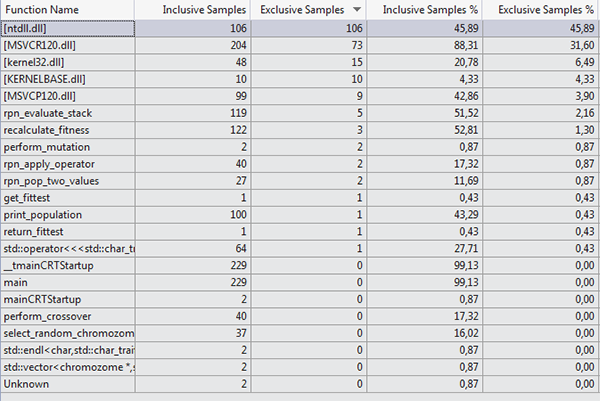
\includegraphics[interpolate,width=1.0\textwidth]{img/prof_flatview.png}
    \caption{Flat view generovaný nástrojem VSPerf}
    \label{obr:flatview}
\end{figure}

\newpage

\section{Hierarchical view}

Hierarchický pohled (také \emph{call tree}, \emph{strom volání}) přidává kontext do předchozího případu. Konkrétně jde o dedukování, která funkce volala kterou, tedy je možné snáze identifikovat možný výkonnostní problém, pokud není přímo ve volané funkci, ale v kontextu okolo.

Tento pohled výrazně rozšiřuje množinu identifikovatelných problémů. Příkladem problému, který odhalí tento pohled navíc oproti \emph{flat view}, je například ten, kdy máme poměrně náročnou funkci, která je volaná z mnoha míst v celém programu. Pokud je ale někde chybně volána častěji, než je nezbytně nutné, bude velké procento volání (popř. vzorků, tráveného času) zvýrazňovat místo problému.

\begin{figure}[h]
    \centering
    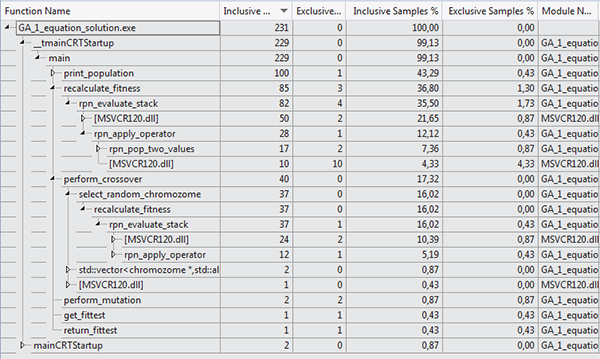
\includegraphics[interpolate,width=1.0\textwidth]{img/prof_calltree.png}
    \caption{Hierarchical view generovaný nástrojem VSPerf}
    \label{obr:hieview}
\end{figure}

\section{Graph view}

Grafový pohled je grafickým vylepšením pohledu hierarchického. Výhodou je možnost vidět všechny vazby naráz, bez duplikace jednotlivých funkcí v několika větvích stromu.

\begin{figure}[H]
    \centering
    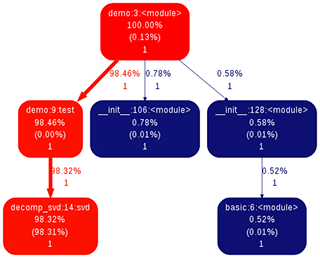
\includegraphics[interpolate,width=0.5\textwidth]{img/prof_graph.png}
    \caption{Graph view s vyznačenou \emph{hot path}, Zdroj: \url{http://claudiovz.github.io/scipy-lecture-notes-ES/advanced/optimizing/index.html} }
    \label{obr:gview}
\end{figure}

V hierarchickém pohledu totiž mohla nastat situace, kdy se v celém stromu jedna funkce vyskytuje na více místech, a to tehdy, pokud je volána z několika jiných funkcí. V grafovém pohledu jsou všechny duplikáty sloučeny do jednoho uzlu a z uzlů představujících volající funkce jsou do něj vedeny hrany.

\section{Object-method view}

V podstatě se jedná o \emph{flat view}, ovšem v modifikaci pro programy psané v objektově orientovaném jazyce. Položky seznamu (zde metody), jsou sdruženy do skupin podle náležitosti třídě. Pokud je program správně dekomponován, lze pomocí tohoto pohledu identifikovat třídu, jejíž metody představují časově nejnáročnější operace.

\begin{figure}[H]
    \centering
    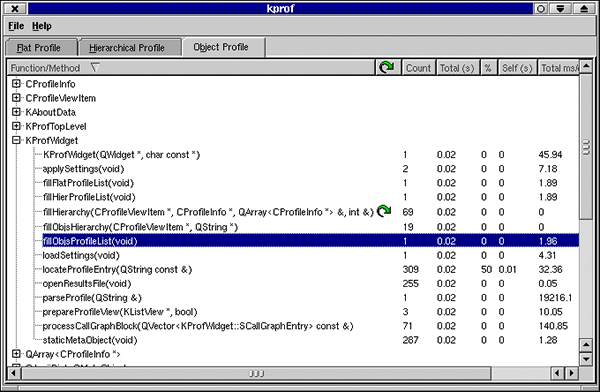
\includegraphics[interpolate,width=0.8\textwidth]{img/prof_objectview.png}
    \caption{Object-method view, Zdroj: \url{http://kprof.sourceforge.net/} }
    \label{obr:objview}
\end{figure}

Výhoda tohoto pohledu může spočívat například v použití pro týmově vyvíjený produkt, kde každou komponentu měl na starosti jiný vývojář. Lze tedy snadno identifikovat osobu zodpovědnou za pomalý běh. Další vlastnosti tento pohled přebírá od \emph{flat view}.

\section{Flame graph}

Tento pohled lze snadno generovat z pohledu hierarchického. Ve své podstatě jde pouze o expandovaný hierarchický pohled, který je uspořádán odspoda (kořen) nahoru (listy). Značnou výhodou je škálování jednotlivých položek podle procentuálních hodnot zkoumané veličiny - tráveného času (zde inkluzivního). Kořen zaujímá $100\%$ šířky grafu, a veškeré volané funkce jsou o úroveň výše, škálované relativně vůči celkovému exkluzivnímu času volající funkce a jsou vyneseny tak, aby zaujímaly přesně takovou procentuální šířku.

Tento druh vizualizace lze považovat za přínosný zejména z toho důvodu, že znáznorňuje poměrný strávený čas vůči všem ostatním volaným funkcím. Tyto poměry nemusí být z hierarchického pohledu vidět. Také tento pohled významně redukuje množství dat a efektivně eliminuje nevýznamné položky - ty mají ve výsledném grafu minimální šířku.

Takový graf ale vzhledem ke své obsáhlosti musí být buď dostatečně velký, nebo interaktivní. Interaktivitu si můžeme představit například možností rozkliknout funkci, která je pro nás zajímavá - poté se změní poměry šířek, vybraná funkce tvoří výchozí bod se $100\%$ šířkou a všechny ostatní jí volané funkce škálujou podle ní.

\begin{figure}[h]
    \centering
    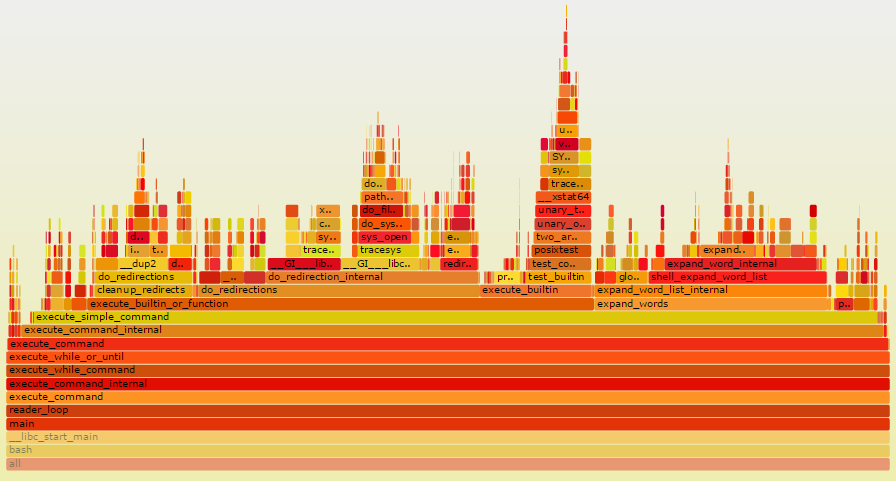
\includegraphics[interpolate,width=1.0\textwidth]{img/prof_flame.png}
    \caption{Flame graph, Zdroj: \url{http://www.brendangregg.com/FlameGraphs/cpuflamegraphs.html} }
    \label{obr:flamegr}
\end{figure}

\subsection{Detailed graph}

Variací \emph{flame graph} pohledu je tzv. detailní pohled. Ten pouze zužuje celkový pohled na výběr třech po sobě jdoucích úrovní. U takového pohledu je tedy nutná jistá interaktivita, která spočívá v možnosti procházet jednotlivé úrovně klikáním. Dále může být připojen výpis programového kódu se zvýrazněnými částmi, které jsou z hlediska výkonu významné.

\begin{figure}[h]
    \centering
    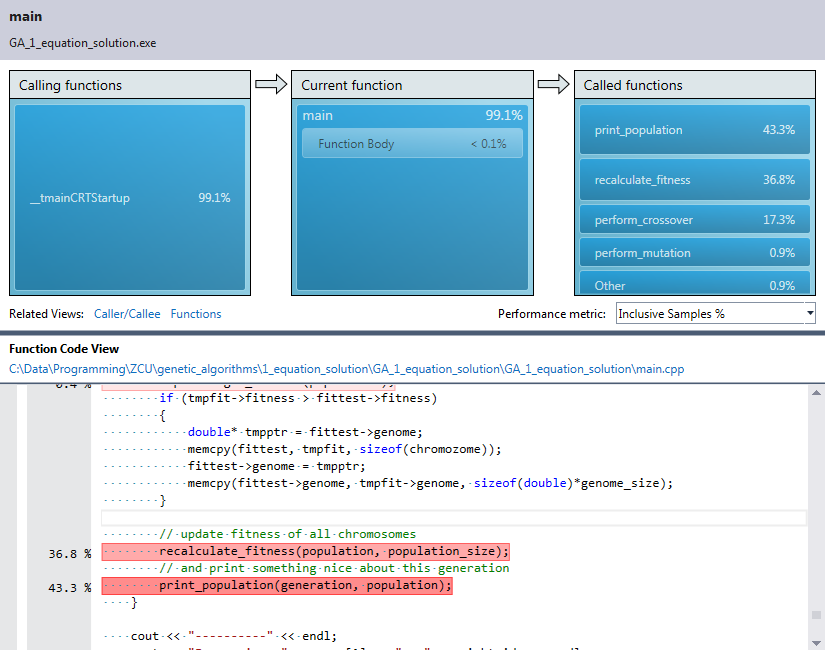
\includegraphics[interpolate,width=1.0\textwidth]{img/prof_detailgraph.png}
    \caption{Detailed view generovaný nástrojem VSPerf}
    \label{obr:detailview}
\end{figure}

\section {Heat maps}

Heat mapy nejsou v současné době příliš rozšířenou technikou vizualizace profilingových dat, ale je možné je pro určité body zájmu aplikovat. Oproti předchozím způsobům dovoluje zobrazovat do určité míry i trojrozměrná data. Vodorovná osa znázorňuje tok času, svislá osa zkoumané body zájmu, v případě profilingu jde o funkce (metody). Osa času je často diskretizovaná na časové úseky větší, než je snímkovací perioda, jelikož je nutné za tento interval nasbírat takový počet výskytů zkoumaného jevu (programový čítač ukazuje na instrukci z instrukčního toku funkce), aby bylo možné rozlišit významnost.

\begin{figure}[h]
    \centering
    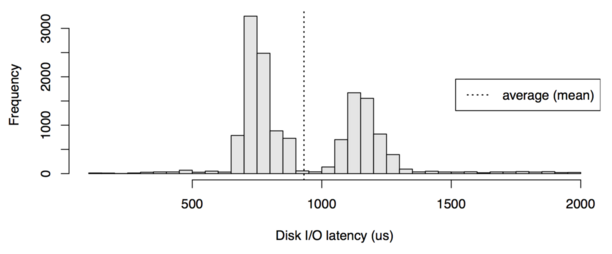
\includegraphics[interpolate,width=1.0\textwidth]{img/prof_histogram.png}
    \caption{Histogram četností dob odezvy pevného disku při čtení a zápisu, Zdroj: \url{http://www.brendangregg.com/HeatMaps/latency.html}}
    \label{obr:heathistoview}
\end{figure}

Na obrázku \ref{obr:heatview} je vidět heat mapa odezvy pevného disku, což je momentálně jeden z hlavních případů použití této techniky. Vodorovná časová osa je rozdělena na diskrétní úseky po 1 vteřině a v rámci tohoto časového úseku bylo provedeno několik stovek čtení. Po uplynulé vteřině byl z časů odezvy vytvořen histogram četností (obrázek \ref{obr:heathistoview}), výšky sloupců byly převedeny na intenzitu barvy, a do výsledného grafu byl takto obarvený sloupec vložen ve vertikálním směru.

\begin{figure}[h]
    \centering
    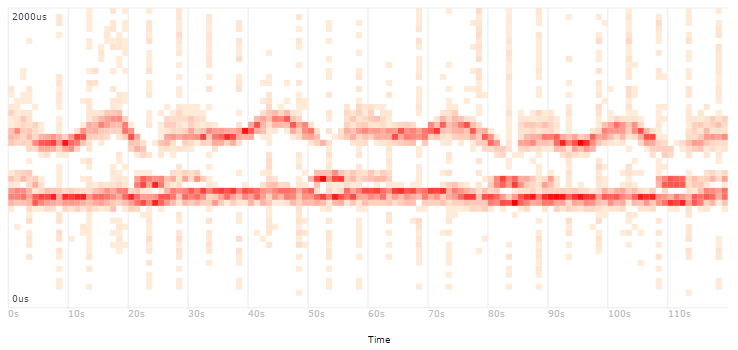
\includegraphics[interpolate,width=0.8\textwidth]{img/prof_heatmap.png}
    \caption{Heat map, Zdroj: \url{http://www.brendangregg.com/HeatMaps/latency.html}}
    \label{obr:heatview}
\end{figure}

Výhodou takového grafu může být zejména viditelnost tendence. Na základě takto viditelných dat je možné posléze odhadovat, jak se bude program chovat při násobně větší zátěži. Určité aplikace totiž nedovolují provádět profiling při vysoké zátěži a to zejména kvůli zpomalení, které profilery způsobují. Příkladem mohou být veškeré služby, u kterých je žádoucí minimální odezva - kromě realtime systémů lze uvést například herní servery pro masově hrané hry, kde může vyšší odezva znamenat zhoršení herního zážitku.

\section{Shrnutí}

Způsobů vizualizace existuje poměrně velké množství, z velké části jde ale o modifikaci nebo kombinaci způsobů výše uvedených. Každý pohled zvýrazňuje trochu jinou informaci, přičemž záleží vždy na konkrétním případu užití, jak je interpretována. Proto je důležité mít k dispozici co možná nejširší škálu různých pohledů.

Také je vhodné řešit, jakým způsobem, tedy pomocí jakého \uv{média} bude výsledek předán vývojáři. Velká část nástrojů poskytuje výsledky v textové formě, čili snadno zobrazitelné kteroukoliv konzolí. Některé nástroje obsahují vlastní GUI, které je ovšem často závislé na platformě nebo grafickém prostředí. Dále malá skupina nástrojů poskytuje možnost exportovat výsledek do nějakého známého obrazového formátu - typicky PNG nebo SVG.

V rámci této práce bude realizován výstup do pohledů \emph{flat view}, \emph{hierarchical view}, \emph{flame graph}, a budou prozkoumány možnosti \emph{heat map} pohledu pro potřeby profilingu. Dále bude zahrnuta vizualizace do formy webové prezentace, tedy za použití technologií HTML, CSS a Javascript. Zároveň bude dodržena podobná modularita jako u vstupů, tedy bude možné kdykoliv přidat další \uv{médium} jen přidáním modulu.


\newpage

\chapter{Dostupné nástroje pro vizualizaci}

Vizualizačních nástrojů existuje také poměrně velké množství. Kritériem výběru by byl určitě podporovaný profiler, jehož data lze nástrojem zpracovávat, dále určitě závislost na platformě, podporované vizualizační techniky a případně další kritéria, jako je například interaktivita.

\section{Visual Studio Performance Profiling}

VSPerf je kombinovaným řešením, tedy obsahuje i vizualizaci nasbíraných dat. Jedná se o uzavřené řešení, podporován je pouze formát samotného profileru z této sady, z čehož opět vyplývá i závislost na prostředí MS Visual Studio a OS MS Windows. Data lze zobrazit pomocí \emph{flat view}, \emph{hierarchical view}, \emph{detailed graph} a dalších, nepříliš významných technik.

Nástroj poskytuje pouze GUI se všemi pohledy, tedy nelze generovat žádná obrazová data, ani jiný přenositelný formát výstupu.

\section{KCachegrind}

Pro nástroje Callgrind a OProfile lze použít vizualizační prostředí KCachegrind. Jedná se o grafické prostředí, které ke svému běhu potřebuje OS GNU/Linux a grafické prostředí KDE, a je schopné vizualizovat data v pohledech \emph{flat view}, \emph{hierarchical view}, \emph{graph view} a něčem, co připomíná \emph{flame graph}.

Kromě GUI umožňuje KCachegrind navíc exportovat grafy do vektorových formátů.

\section{KProf}

Tento nástroj je velmi podobný nástroji předchozímu, jen dovede zpracovávat data nástroje \emph{gprof} a jemu podobných. Také se jedná o grafické prostředí vyžadující OS GNU/Linux a grafické prostředí KDE. Implementuje pohledy \emph{flat view}, \emph{hierarchical view}, \emph{graph view} a \emph{object-method view}. Jedná se o podstatně jednodušší prostředí, než kterékoliv výše uvedné, ale pohledy nejsou ochuzeny o nic podstatného.

Tento nástroj poskytuje pouze GUI, opět tedy není přítomna žádná možnost, jak zpracovaná data přenést na jinou platformu.

\section{GProf2dot}

Poměrně cenným nástrojem v oblasti vizualizace profilingových dat je \emph{gprof2dot}. Původně dokázal zpracovat pouze výstupy nástroje \emph{gprof}, postupně byla podpora rozšířena na širokou škálu profilerů zahrnujících \emph{perf}, \emph{OProfile}, \emph{callgrind}, i například \emph{Very Sleepy}. Jelikož se jedná o skript psaný v jazyce Python, jeho přenositelnost je podmíněná existencí interpretu pro danou platformu, a také několika málo závislostmi. Oficiálně jsou podporovány OS MS Windows a GNU/Linux. Výstupem je vždy pouze \emph{graph view}, který lze poměrně ve velké míře přizpůsobovat.

Nástroj sice neposkytuje GUI, zato výstupem je obrázek v rastrovém nebo vektorovém formátu.

\section{RotateRight Zoom}

Podobně jako VSProf je i RotateRight Zoom kombinovaným uzavřeným řešením. Dokáže tedy zpracovávat pouze data nashromážděná vlastním profilerem. Oproti předchozím nástrojům má tu výhodu, že lze vizualizovat data na kterékoliv z nejpoužívanějších platforem. Ačkoliv není podporován profiling na OS MS Windows, existuje pro něj grafické rozhraní, které dovoluje zobrazovat data z profilingu probíhajícího na vzdáleném serveru. Kromě \emph{flat view} a \emph{hierarchical view} implementuje i pohled \emph{timeline}, tedy časové osy.

Nástroj obsahuje GUI a zároveň je možné exportovat data do textového formátu.

\section{Shrnutí}

Dostupné nástroje často buď neposkytují přenositelnost výstupu, neobsahují potřebné pohledy, nebo nepodporují širší škálu profilerů.

Obsahem následující kapitoly bude návrh takového nástroje, který poskytne vysokou přenositelnost výstupu, velký výběr pohledů na profilingová data a zároveň zaručenou podporu pro velké množství profilerů, resp. jejich výstupních formátů. V rámci této práce bude realizováno jádro takového nástroje, a implementace pouze vybraných vstupních a výstupních modulů.



\newpage

\chapter{Návrh nástroje}

Účelem nástroje bude načítat profilingová data z výstupních souborů známých profilerů, analyzovat je a následně vizualizovat pomocí vybraného výstupního modulu. Jedním z hlavních požadavků je i modularita nástroje, která bude spočívat ve členění na tři hlavní skupiny modulů, jak je znázorněno na obrázku \ref{obr:systemmodules}. První částí je pevný základ, tedy samotná spustitelná část. Ta bude přejímat požadavky od uživatele, vybírat vstupní modul, analyzovat data a předávat je výstupnímu modulu. Druhou skupinou jsou vstupní moduly - pro každý formát bude existovat právě jeden vstupní modul. Tyto moduly se budou starat o načtení dat, transformaci do jednotné formy a předání zpět do jádra nástroje. Poslední skupinou jsou výstupní moduly, kterým jsou předána analyzovaná data opět v jednotné formě. Tyto moduly na základě vstupních parametrů od uživatele poskytnou požadovaný výstup.

Aplikace bude pouze konzolová. Tím je odbourána závislost na jakémkoliv grafickém prostředí.

\begin{figure}[h]
    \centering
    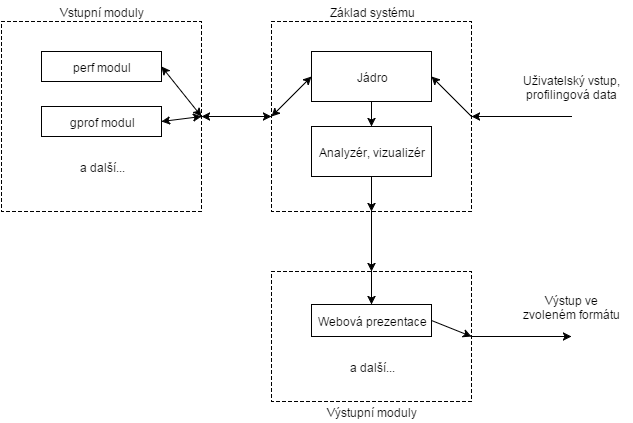
\includegraphics[interpolate,width=1.0\textwidth]{img/system_diagr.png}
    \caption{Architektura nástroje, rozdělení do třech hlavních skupin modulů}
    \label{obr:systemmodules}
\end{figure}

\section{Základ systému}

Tato skupina modulů bude představovat spustitelný program. Moduly základu budou tedy pevně svázány po čase kompilace, tedy nebudou fyzicky oddělitelné. To z důvodu, že je nutné mezi nimi zajistit maximální kompatibilitu, kterou lze do jisté míry zaručit při sestavení.

\subsection{Jádro}

Hlavním úkolem jádra bude obstarávat propojení všech modulů, které budou zapojeny do procesu zpracování vstupů, analýzy a následně formátování výstupu. Samotné jádro bude mít znalost pouze rozhraní se vstupními moduly a s analyzérem, kterému předá zpracovaná data ze vstupních modulů.

Jádro bude představovat i vstupní bod programu, tedy bude přejímat parametry příkazové řádky a na základě nich vybírat příslušné moduly a parametry vizualizace. Také se bude starat o logovací výstupy, které bude možné tisknout buď do konzole, nebo přesměrovat do souboru.

\subsection{Analyzér}

Tento modul bude na vstupu očekávat dostupná profilingová data v normalizovaném formátu, která bude analyzovat a tvořit z nich datové struktury pro jednotlivé pohledy. Bude tedy zodpovědný za první část sestavení pohledů. Druhá část bude implementována až v samotném výstupním modulu, který pouze přečte naformátované datové struktury a vytvoří z nich konkrétní pohled.

Analyzér nesmí předpokládat existenci veškerých dat, jelikož ne každý profiler poskytuje stejnou škálu informací. Od toho se bude odvíjet i množina pohledů, které je schopen předzpracovat a předat výstupnímu modulu k vizualizaci.

\section{Vstupní moduly}

Vstupní moduly jsou takové knihovny, které odděleně od sebe implementují jednotlivé formáty výstupních souborů profilerů. Jejich úkolem je na základě vstupního souboru (popř. adresáře) načíst data nashromážděná profilerem, normalizovat je do jednotného formátu a předat je jádru. 

Veškeré vstupní moduly budou zrealizovány jako dynamické knihovny, na jejichž existenci nesmí spuštění programu záviset, vyjma případu, kdy je vyžadováno zpracování formátu, jehož zpracování tento modul implementuje.

\section{Výstupní moduly}

Tyto moduly budou mít na starost implementaci specifických způsobů vizualizace předzpracovaných dat, tedy konkrétní technologii. Budou přejímat normalizovaná data dostupných způsobů vizualizace profilingových dat od analyzéru. Nesmí ale předpokládat existenci dat pro všechny pohledy, a to ze stejného důvodu, jako analyzér - profiler nemusel potřebná data poskytnout.

Výstupní moduly budou stejně jako vstupní realizovány jako nezávislé dynamické knihovny.

\section{Technologie}

Nástroj bude realizován jako přenositelný. Jeho zdrojový kód bude psán v jazyce C++, a to proto, že je snadno zkompilovatelný na většině platforem bez nutnosti instalovat nestandardní závislosti, a jeho kompilátor je zpravidla součástí výbavy každého serverového systému. Také se jedná o objektově orientovaný jazyk, takže bude možné psát čitelný a snadno rozšiřitelný kód, který bude strukturou odpovídat výše uvedenému návrhu.

Pro správu zdrojových kódů bude použit systém správy verzí \emph{git}.

Použití dalších technologií je závislé na implementačních detailech. V rámci navazující bakalářské práce bude například použita základní škála frontendových webových technologií pro vizualizaci profilingových dat formou webové prezentace. Jde o technologie HTML, CSS a Javascript. Webová prezentace je dobrým příkladem snadno interpretovatelné formy vizualizace, která je podporována napříč širokou škálou platforem od standardních počítačů až po mobilní zařízení, a to bez rozdílu operačního systému.

\section{Licence}

Nástroj bude vyvíjen jako svobodný software pod licencí GNU GPLv3 \cite{gplv3}. Důvodem je možnost otevřít vývoj široké veřejnosti. Takový nástroj ani není vhodné uzavírat co se vývoje týče, jelikož existuje příliš velké množství profilerů, vizualizačních technik a možných technologií pro vizualizaci. Zapojením široké vývojářské veřejnosti může dojít k podstatnému zlepšení kvality a obsáhlosti nástroje.

\section{Shrnutí}

Byl navržen modulární nástroj, který bude řešit problémy uvedené v předchozích kapitolách. Jedná se zejména o přenositelnost výstupu nástroje a sjednocení vizualizace pro různé profilery. Dále jde o přenositelnost samotného programu, jeho modularitu, která úzce souvisí s rozšiřitelností a v neposlední řadě i o otevření zdrojových kódů veřejnosti.

Vývoj tohoto nástroje se předpokládá v rámci bakalářské práce.



\newpage

\chapter{Závěr}

Cílem této práce bylo analyzovat dostupné profilingové nástroje, způsoby vizualizace dat jimi nasbíraných a navrhnout takový nástroj, který bude umět načíst formáty různých profilerů, zpracovat je a vytvořit pohled, který nebude závislý na platformě.

Problematika profilingu je poměrně rozsáhlá, a to díky tomu, že výkonnostní analýzu bylo žádoucí provádět již od počátků moderních systémů. Za tu dobu bylo vyvinuto velké množství různých profilerů a byly ustáleny standardní pohledy z profilingových dat generované. Analýza obsahuje nástroje, které se řadí mezi obecně nejpoužívanější. Z nich byly vybrány dva, které budou v rámci bakalářské práce implementovány do výsledného nástroje. Také je obsažena analýza nejčastěji používaných vizualizačních technik, ze kterých byly vybrány tři pro implementaci, a jedna k analýze možností pro vizualizaci takových dat.

V poslední části byl navržen nástroj, který bude realizován v rámci bakalářské práce. Výsledkem bude modulární přenositelná aplikace, která bude implementovat vstupní moduly pro načtení výstupních formátů nástrojů \emph{perf} a \emph{gprof}, a výstupní modul pro vizualizaci pomocí standardních webových technologií.

Osobně pro mě práce byla přínosná hlavně díky znalostem, které jsem v průběhu psaní získal. Poskytla mi přehled o existujících profilerech, způsobech získávání dat a také o vizualizačních technikách. V minulosti jsem se s profilingem setkal pouze v omezené míře, a tak tato práce zahrnovala i velké množství studia.



\newpage

\bibliographystyle{csplainnat}
\bibliography{bakalarka}






%% Seznam zkratek

\newenvironment{seznamzkratek}[1]%
  {%
    \chapter*{Seznam zkratek}
    \addcontentsline{toc}{chapter}{Seznam zkratek}
    \begin{acronym}[#1]
  }{%
    \end{acronym}
    \newpage
  }%
\newcommand{\novazkratka}[3]%
  {\acro{#1}[#2]{#3}}
\newcommand{\zkratka}[1]%
  {\ac{#1}}
\newcommand{\zk}[1]%
  {\acs{#1}}
\newcommand{\zkratkatext}[1]%
  {\acl{#1}}

\begin{seznamzkratek}{PROF}

\novazkratka{zkIRQ}{IRQ}{Interrupt Request - vnější hardwarové přerušení}
\novazkratka{zkHPC}{HPC}{Hardware Performance Counters - hardwarové výkonnostní čítače}
\novazkratka{zkNMI}{SSD}{Solid-state drive - disková jednotka založená nejčastěji na nevolatilní flash paměti}
\novazkratka{zkNMI}{NMI}{Non-maskable interrupt - nemaskovatelné přerušení}
\novazkratka{zkOS}{OS}{Operační systém}
\novazkratka{zkCPU}{CPU}{Central processing unit - hlavní výpočetní jednotka počítače}
\novazkratka{zkPC}{PC}{Program counter - instrukční čítač v rámci programu, obsahuje offset instrukce k provedení}
\novazkratka{zkOS}{CSV}{Comma-separated values - formát souboru s buňkami oddělenými specifickým znakem (čárka, středník, aj.)}
\novazkratka{zkHTML}{HTML}{HyperText Markup Language - značkovací jazyk používaný pro webové stránky}
\novazkratka{zkCSS}{CSS}{Cascading Style Sheets - kaskádové styly používané pro webové stránky}

\end{seznamzkratek}

\end{document}




























